\documentclass[12pt]{article}
\usepackage[utf8]{inputenc}
\usepackage{graphicx}
\usepackage{amsmath}
\usepackage{amssymb}
\usepackage{amsthm}
\usepackage[top=1in, bottom=1in, left=1in, right=1in]{geometry}

\begin{document}

\begin{center}
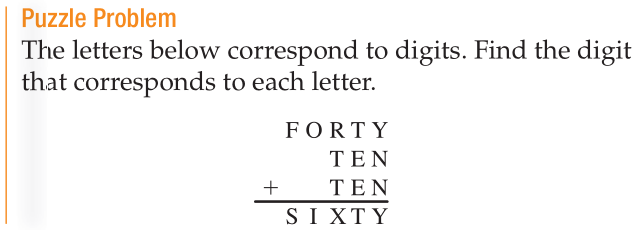
\includegraphics[scale=0.6]{forty.png}
\end{center}

\noindent\textit{Solution.}
Starting with the last column, we have
\begin{align*}
    Y+N+N&=10a+Y\\
    N=5a
\end{align*}
where $a=1$ or $a=0$, since $N$ is a single digit number.
\vspace{20px}

\noindent\textit{Case 1.} $a=1$. Plugging this into the previous equation, we get
\[N=5a=5(1)=5.\]
Going to the fourth column, since we have to carry a $1$, we have
\begin{align*}
    1+T+E+E&=10b+T\\
    2E&=10b-1
\end{align*}
where $b\in\mathbb{Z}$. However, this is a contradiction since $10b-1$ is not even. Therefore, $a\neq 1$.
\vspace{20px}

\noindent\textit{Case 2.} $a=0$. Plugging this into the same equation as in \textit{Case 1}, we get
\[N=5a=5(0)=0.\]
Going to the fourth column, since we do not carry a $1$, we have
\begin{align*}
    T+E+E&=10b+T\\
    E&=5b
\end{align*}
where $b=1$ or $b=0$, since $E$ is a single digit number. If $b=0$, we get
\[E=5b=5(0)=0.\]
However, we already have $N=0$. Therefore, $b=1$ so
\[E=5b=5(1)=5.\]
Hence, $\boxed{N=0}$ and $\boxed{E=5}$.
\newpage

\noindent Since $F\neq S$, we must carry a number to the first column. To find this number, notice that
\[\max(ORTY+TEN+TEN)=9999+999+999<20000.\]
This means we must carry a $1$ to the first column. Therefore,
\[S=F+1.\]
Similarly, since $O\neq I$, we must carry a number to the second column. To find this number, notice that
\[\max(RTY+TEN+TEN)=999+999+999<3000.\]
This means we must carry a $1$ or a $2$ to the second column. Therefore, there are two cases we must look at.
\vspace{20px}

\noindent\textit{Case 1.} Carry a $1$. This yields
\begin{align*}
    1+O&=10+I\\
    O&=9+I.
\end{align*}
The $10$ came from the fact that we are carrying a $1$ to the first column. Now, since $O$ is a single digit number, it must be the case that $I=0$. However, we already have $N=0$, so this is a contradiction. Therefore, we must carry a $2$.
\vspace{20px}

\noindent\textit{Case 2.} Carry a $2$. This yields
\begin{align*}
    2+O&=10+I\\
    O&=8+I.
\end{align*}
Now, since $O$ is a single digit number, it must be the case that $I=0$ or $I=1$. However, we already have $N=0$. Thus, $I=1$. Therefore
\[O=8+I=8+1=9.\]
Hence, $\boxed{I=1}$ and $\boxed{O=9}$.
\newpage

\noindent Looking at the fourth column, since $E=5$, we have
\[\max(T+E+E)=\max(T+5+5)=9+5+5=19.\]
Therefore, we must carry a $1$ to the third column. This yields
\begin{align*}
    1+R+T+T&=20+X\\
    1+R+2T&=20+X\\
    R&=X-2T+19.
\end{align*}
The $20$ came from the fact that we are carrying a $2$ to the second column. Now we have an equation for $R$. To digest this equation, let us look at all of the possibilities for $T$. First of all, it must be the case that
\[1+R+T+T=1+R+2T\geq 20.\]
This is since the sum must be at least $20$ to carry a $2$ to the second column.
\vspace{20px}

\noindent\textit{Case 1.} $T=0$, $T=1$, $T=5$, or $T=9$. Any of these $T$ values violate the values of $N$, $E$, $I$, and $O$. Therefore, $T\neq 0$, $T\neq 1$, $T\neq 5$, and $T\neq 9$.
\vspace{20px}

\noindent\textit{Case 2.} $T\in\mathbb{Z}$ such that $2\leq T\leq 4$. We have
\[\max(1+R+2T)=1+9+2(4)=18<20.\]
This means the sum is not big enough to carry a $2$ to the second column. Therefore, $T$ cannot be $2\leq T\leq 4$.
\vspace{20px}

\noindent\textit{Case 3.} $T=6$. We have
\[\max(1+R+2T)=\max(1+R+2(6))=\max(R+13)=9+13=22\geq 20.\]
This means the sum is big enough to carry a $2$ to the second column. Since this inequality holds for $T=6$, it will also hold for any $T>6$. Thus, this inequality holds for \textit{Case 4} and \textit{Case 5}. Now, using the equation that we derived for $R$, we get
\begin{align*}
    R&=X-2T+19\\
    R&=X-2(6)+19\\
    R&=X+7.
\end{align*}
First of all, $X\neq 0$ and $X\neq 1$ since we already have $N=0$ and $I=1$. Next, if $X=2$, we get
\[R=X+7=2+7=9.\]
However, $R\neq 9$ since we already have $O=9$. Finally, if $X\geq 3$, we get
\[R=X+7\geq 3+7=10.\]
However, $R$ must be a single digit number. Therefore, by way of contradiction, we have $T\neq 6$.
\newpage

\noindent\textit{Case 4.} $T=7$. Using the equation that we derived for $R$, we get
\begin{align*}
    R&=X-2T+19\\
    R&=X-2(7)+19\\
    R&=X+5.
\end{align*}
First of all, $X\neq 0$ and $X\neq 1$ since we already have $N=0$ and $I=1$. Next, if $X=2$, we get
\[R=X+5=2+5=7.\]
However, $R\neq 7$ since we already have $T=7$. Next, if $X=4$, we get
\[R=X+5=4+5=9.\]
However, $R\neq 9$ since we already have $O=9$. Next, if $X\geq 5$, we get
\[R=X+5\geq 5+5=10.\]
However, $R$ must be a single digit number. Finally, if $X=3$, we get
\[R=X+5=3+5=8.\]
Thus, $R=8$. Now, to see if these values of $T$, $X$, and $R$ work, we look at the list of values that we found out for each variable. We have $N=0$, $E=5$, $I=1$, $O=9$, $T=7$, $X=3$, and $R=8$. Ordering these values, we get
\[0,1,3,5,7,8,9.\]
From the equation that we derived earlier,
\[S=F+1,\]
we must have a gap of $3$. This is since, for instance, if $F=2$, we would get \[S=F+1=2+1=3.\]
However, $3$ is already occupied by another variable. Therefore, by way of contradiction, we have $T\neq 7$.
\newpage

\noindent\textit{Case 5.} $T=8$. Using the equation that we derived for $R$, we get
\begin{align*}
    R&=X-2T+19\\
    R&=X-2(8)+19\\
    R&=X+3.
\end{align*}
First of all, $X\neq 0$, $X\neq 1$, and $X\neq 5$ since we already have $N=0$, $I=1$, and $E=5$. Next, if $X=2$, we get
\[R=X+3=2+3=5.\]
However, $R\neq 5$ since we already have $E=5$. Next, if $X=6$, we get
\[R=X+3=6+3=9.\]
However, $R\neq 9$ since we already have $O=9$. Next, if $X\geq 7$, we get
\[R=X+3\geq 7+3=10.\]
However, $R$ must be a single digit number. Finally, there are two more cases: $X=3$ and $X=4$.
\vspace{20px}

\noindent\textit{Case 5a.} $X=3$. We have
\[R=X+3=3+3=6.\]
Thus, $R=6$. Now, to see if these values of $T$, $X$, and $R$ work, we look at the list of values that we found out for each variable. We have $N=0$, $E=5$, $I=1$, $O=9$, $T=8$, $X=3$, and $R=6$. Ordering these values, we get
\[0,1,3,5,6,8,9.\]
From the equation that we derived earlier,
\[S=F+1,\]
we must have a gap of $3$. However, there is no gap of $3$. Therefore, by way of contradiction, we have $X\neq 3$.
\vspace{20px}

\noindent\textit{Case 5b.} $X=4$. We have
\[R=X+3=4+3=7.\]
Thus, $R=7$. Now, to see if these values of $T$, $X$, and $R$ work, we look at the list of values that we found out for each variable. We have $N=0$, $E=5$, $I=1$, $O=9$, $T=8$, $X=4$, and $R=7$. Ordering these values, we get
\[0,1,4,5,7,8,9.\]
From the equation that we derived earlier,
\[S=F+1,\]
we must have a gap of $3$. The gap of $3$ happens between $1$ and $4$. Thus, $F=2$. This implies
\[S=F+1=2+1=3.\]
Therefore, $\boxed{T=8}$, $\boxed{X=4}$, $\boxed{R=7}$, $\boxed{F=2}$, and $\boxed{S=3}$.
\newpage

\noindent The last variable we must find is $Y$. The variables that we found are $N=0$, $E=5$, $I=1$, $O=9$, $T=8$, $X=4$, $R=7$, $F=2$, and $S=3$. Ordering these values, we get
\[0,1,2,3,4,5,7,8,9.\]
The missing digit it $6$. Thus, $Y=6$. Therefore, the answer is \[\boxed{N=0},\boxed{I=1},\boxed{F=2},\boxed{S=3},\boxed{X=4},\boxed{E=5},\boxed{Y=6},\boxed{R=7},\boxed{T=8},\boxed{O=9}.\]
To see if this is correct, we plug in the values,
\begin{align*}
    FORTY&=29786\\
    TEN&=850\\
    SIXTY&=31486,
\end{align*}
and check the sum,
\begin{align*}
    FORTY+TEN+TEN&=29786+850+850\\
    &=31486\\
    &=SIXTY.
\end{align*}
\qed

\end{document}